\section{Usuario}
\subsection{Representación}
Un usuario quedará identificado por su \textit{idUser}, los usuarios se guardarán en una carpeta especial con ficheros como el siguiente.
\lstinputlisting[caption=0.usr]{../.chatConfig/users/0.usr}
La estructura del fichero es la siguiente
\begin{itemize}
	\item Identificador de usuario
	\item Nombre de usuario
	\item Contraseña
	\item Grupos a los que pertenece
\end{itemize}

Esta configuración permite tener un chat con nosotros mismos.
Existirán funciones para cargar y guardar usuarios en ficheros.


\subsection{Mensajes}
Cada usuario tiene una instancia de la clase \textit{Printer} que recibirá y mostrará los mensajes.
Los mensajes tienen un identificador del grupo al que pertenecen, del usuario que los envía y un identificador del mensaje.
Estos tres parámetros nos permitirán identificar de forma única cada mensaje.

\begin{figure}[H]
	\centering
	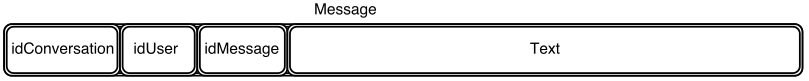
\includegraphics[width=0.8\textwidth]{./Imagenes/message.png}
\end{figure}

Un fichero de conversación será una sucesión de mensajes, como muestra el siguiente ejemplo.

\lstinputlisting[caption=example.chat]{../.chatConfig/conversations/example.chat}

Los números al inicio son el identificador de conversación, el del usuario que manda el mensaje y el identificador de su mensaje.
Estos tres números en conjunto formarán el identificador de cada mensaje.